% "Maths encyclopedia kit": one source exercising the whole default preamble.
% No \documentclass is needed - DocsForge wraps bare diagram sources in a
% standalone document with amsmath, amssymb, tikz, pgfplots, tikz-cd and
% tkz-euclide preloaded.

% 1. Commutative diagram (tikz-cd)
\begin{tikzcd}
  \mathbb{R}^2 \ar[r, "f"] \ar[d, "g"'] & \mathbb{R}^3 \ar[d, "h"] \\
  \mathbb{R} \ar[r, "k"']               & \mathbb{R}
\end{tikzcd}

% 2. Function plot (pgfplots)
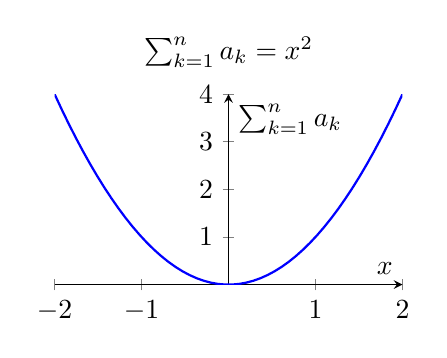
\begin{tikzpicture}
  \begin{axis}[
      width=6cm, height=4cm, axis lines=center,
      xlabel=$x$, ylabel={$\sum_{k=1}^{n} a_k$},
      title={$\sum_{k=1}^{n} a_k = x^2$}
    ]
    \addplot[domain=-2:2, samples=50, thick, blue] {x^2};
  \end{axis}
\end{tikzpicture}

% 3. Euclidean construction (tkz-euclide)
\begin{tikzpicture}
  \tkzDefPoint(0,0){A}
  \tkzDefPoint(4,0){B}
  \tkzDefPoint(0,3){C}
  \tkzDrawSegments(A,B B,C C,A)
  \tkzMarkRightAngle(B,A,C)
  \tkzLabelPoints[below left](A)
  \tkzLabelPoints[below right](B)
  \tkzLabelPoints[above](C)
\end{tikzpicture}